\documentclass[12pt,a4paper]{article}
\usepackage{graphicx}
\usepackage{wrapfig}

\title{Praktikum Physik - Beugung}
\author{Simon Marti, Patricia Schwab, Mirco Kocher}
\date{16.03.2012}

\parindent=0pt 
\begin{document}
\maketitle

%%
% Ziel
%%
\section*{Ziel}

%%
% Motivation
%%
\section*{Motivation}

%%
% Theorie
%%
\section*{Theorie}
Beugungswinkel an Gitter
\begin{equation}
sin\varphi = n\cdot \frac{\lambda}{g}
\end{equation}

Energie eines Photons
\begin{equation}
E = \frac{h\cdot c}{\lambda}
\end{equation}

Bindungsenergie eines Elektrons im $n$-ten Orbit
\begin{equation}
E_n = \frac{-12.6\mbox{eV}}{n^2}
\end{equation}

%%
% Experiment 1
%%
\section*{Experiment I}

% Aufbau und Ablauf
\subsection*{Aufbau und Ablauf}
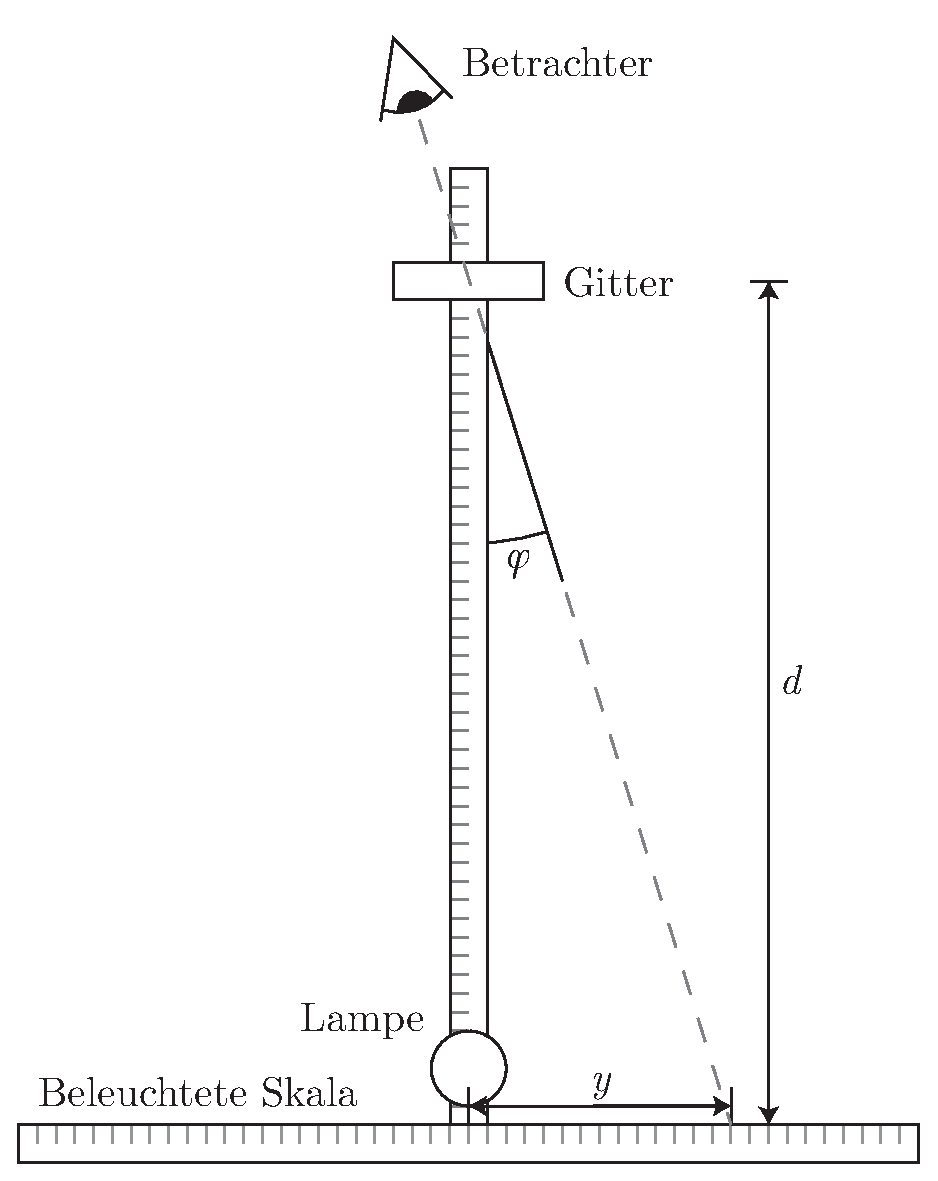
\includegraphics[width=13cm]{illustration.pdf}

Eine Heliumlampe wird auf einer Schine direkt vor eine senkrecht zu Schiene stehende, beleuchtete Skala montiert. Etwas entfernt von der Lampe wird auf der Schiene ein optisches Gitter so montiert, dass ein Betrachter durch das Gitter die Lampe und dahinter die Skala sehen kann.

Der Betrachter (Simon) sieht nun durch das Gitter auf die Skala und sollte darauf mehrere farbige Beugungslinien sehen. Um die Abstand $y$ der Linien besser bestimmen zu k\"onnen f\"ahrt ein Gehilfe (Mirco) mit der Spitze eines Kugelschreibers \"uber die Skala bis sich diese mit einer der Beugungslinien \"uberlagert, was der Betrachter bekanntgibt. Da sich die Position der Beugungslinien je nach Blickwinkel des Betrachters ver\"andern kann wird jeweils der minimale und der maximale Abstand gemessen der gerade noch sichtbar ist.

Aus den gemessenen Abst\"anden $y$ kann nun die Gitterkonstante nach Formel ??? ausgerechnet werden. Zus\"astzlich wird mit einem Mikroskop das Gitter betrachtet und die Gitterkonstante durch abz\"ahlen bestimmt.

% Rohdaten
\subsection*{Rohdaten}
\subsubsection*{Experiment}
\begin{tabular}{|l|l|l|}
\hline
$\lambda$ [A]&$y_{min} [cm]$&$y_{max} [cm]$\\
\hline
7065&22.1&22.7\\
6678&23.7&24.6\\
5875&25.1&25.7\\
5015&25.8&26.5\\
4921&30.7&31.7\\
4713&36.1&37.4\\
4471&38.7&40.0\\
\hline
\end{tabular}\vspace{10pt}

Abstand $d$ = 80cm

\subsubsection*{Mikroskop}
Anzahl Gitterlinien in einer Einheit des Mikroskops: 12

G\"osse dieser Einheit: 0.0208mm

% Auswertung
\subsection*{Auswertung}
\[ g = \frac{\lambda}{sin(tan^{-1}(\frac{y}{d}))} \]

%%
% Experiment 2
%%
\section*{Experiment II}

% Aufbau und Ablauf
\subsection*{Aufbau und Ablauf}
Im Aufbau von Experiment I wird die Heliumlampe durch eine Wasserstofflampe ersetzt und erneut der Abstand $y$ der Beugungslinien gemessen. Die einzigen beiden sichtbaren Beugungslinien die in diesem Versuch sind blau und rot.

Aus den beiden Abst\"anden $y$ wird die Wellenl\"ange der jeweiligen Farbe der Beugungslinien berechnet und daraus kann dann bestimmt werden durch welche Elektronenspr\"unge diese erzeugt worden sind.

% Rohdaten
\subsection*{Rohdaten}
\subsubsection*{Rot}
$y_{min}$ = 34.6cm

$y_{max}$ = 35.4cm

\subsubsection*{Blau}
$y_{min}$ = 24.5cm

$y_{max}$ = 25.4cm

% Auswertung
\subsection*{Auswertung}


%%
% Diskussion
%%
\section*{Diskussion}


\end{document}